\subsection{Support of a measure}

Let \(\mu\) be a measure on a locally compact space \(X\) , and let \(\mathfrak{G}\) be the set of open sets \(U \subset X\) such that the restriction of \(\mu\) to \(U\) is zero; it follows at once from the principle of localization (No.~1, Cor. of Prop. 1) that if \(U_0\) is the union of the sets \(U \in \mathfrak{G}\) , then \(U_0\) itself belongs to \(\mathfrak{G}\) and is therefore the largest of the sets of \(\mathfrak{G}\) .

DEFINITION 1. --- If \(\mu\) is a measure on a locally compact space \(X\) , one defines the support of \(\mu\) , denoted \(\operatorname{Supp}(\mu)\) , to be the closed set complementary to the largest of the open sets in \(X\) on which the restriction of \(\mu\) is zero.

To say that a point \(x \in X\) does not belong to the support of \(\mu\) means that there exists an open neighborhood V of x such that the restriction of \(\mu\) to V is zero; to say that x belongs to the support of \(\mu\) therefore means that for every neighborhood V of x, there exists a function \(f \in \mathcal{K}(X; \mathbf{C})\) , whose support is contained in V, such that \(\mu(f) \neq 0\) .

Examples. --- 1) For a measure on X to be zero, it is necessary and sufficient that its support be empty.

\begin{enumerate}
\def\labelenumi{\arabic{enumi})}
\setcounter{enumi}{1}
\item
  The support of Lebesgue measure on \(\mathbf{R}\) is the entire line \(\mathbf{R}\) ; for, it is nonempty and is invariant under every translation.
\item
  On the interval \(\mathrm{X} = [0,1]\) of \(\mathbf{R}\) consider a countable dense subset, arranged into a sequence \((a_n)\) , and let \(\mu\) be the measure defined by placing the mass \(2^{-n}\) at the point \(a_n\) for every \(n \geqslant 0\) (§1, No.~3, Example I). The support of \(\mu\) is all of \(\mathrm{X}\) ; for, let \(x\) be any point of \(\mathrm{X}\) , \(\mathrm{V}\) a neighborhood of \(x\) , and \(f\) a continuous real-valued function \(\geqslant 0\) on \(\mathrm{X}\) , equal to 1 at the point \(x\) , whose support is contained in \(\mathrm{V}\) (§1, No.~2, Lemma 1); the set of \(y \in \mathrm{V}\) such that \(f(y) > 0\) is open in \(\mathrm{X}\) , therefore contains a point \(a_n\) , consequently \(\mu(f) \geqslant f(a_n)2^{-n} > 0\) .
\end{enumerate}

PROPOSITION 2. --- The support of a measure \(\mu\) is identical to the support of the measure \(|\mu|\) ; if \(\mu\) is real, its support is the union of the supports of the measures \(\mu^{+}\) and \(\mu^{-}\) .

For, if the restriction of \(\mu\) to an open set U is zero, then so is that of \(|\mu|\) (resp. of \(\mu^{+}\) and \(\mu^{-}\) when \(\mu\) is real), and conversely.

\pandocbounded{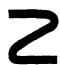
\includegraphics[keepaspectratio]{images/part001_dfbe8ad7.jpg}}

Note that the supports of \(\mu^{+}\) and \(\mu^{-}\) can be nonempty and identical (cf.~Ch. V, § 5, Exer. 5).

PROPOSITION 3. --- If \(\mu\) and \(\nu\) are two measures on a locally compact space X such that \(|\mu| \leqslant |\nu|\) , then \(\operatorname{Supp}(\mu) \subset \operatorname{Supp}(\nu)\) .

For, if the restriction of \(\nu\) to an open set is zero, then so is that of \(\mu\) .

PROPOSITION 4. --- The support of the sum of two measures is contained in the union of their supports.

For, if the restrictions of two measures to an open set are zero, then the same is true of the restriction of their sum.

If \(\mu\) and \(\nu\) are two positive measures, then the support of \(\lambda = \mu + \nu\) is equal to the union of the supports of \(\mu\) and \(\nu\) ; for, if \(x_0\) is a point of the union and V is any neighborhood of \(x_0\) , then there exists a continuous function \(f \geqslant 0\) with support contained in V and such that one of the numbers \(\mu(f)\) , \(\nu(f)\) is \(>0\) ; a fortiori, \(\lambda(f) = \mu(f) + \nu(f) > 0\) .

PROPOSITION 5. --- The support of the restriction of a measure \(\mu\) to an open set U is the trace on U of the support of \(\mu\) .

The proposition is obvious from the definitions.

PROPOSITION 6. --- The set of measures on a locally compact space X, whose support is contained in a closed set F, is a vaguely closed linear subspace of \(\mathcal{M}(\mathrm{X};\mathbf{C})\) .

For, it is the intersection of the vaguely closed hyperplanes with equation \(\mu(f) = 0\) , where f runs over the set of functions in \(\mathcal{K}(\mathrm{X};\mathbf{C})\) whose support does not intersect F.

Suppose X is not compact: given a filter \(\Phi\) on the space \(\mathcal{M}(\mathrm{X};\mathbf{C})\) of measures on X, we shall say that the support of a measure \(\mu\) recedes indefinitely along \(\Phi\) if, for every compact subset K of X, there exists a set \(M\in\Phi\) such that \(\operatorname{Supp}(\mu)\cap K=\varnothing\) for every measure \(\mu\in M\) .

PROPOSITION 7. --- If \(\Phi\) is a filter on \(\mathcal{M}(\mathrm{X};\mathbf{C})\) such that the support of \(\mu\) recedes indefinitely along \(\Phi\) , then \(\mu\) converges vaguely to 0 with respect to \(\Phi\) .

Let \(f\) be any function in \(\mathcal{K}(\mathrm{X};\mathbf{C})\) and let \(K\) be its support. By hypothesis, there exists a set \(M \in \Phi\) such that for every measure \(\mu \in M\) , \(\operatorname{Supp}(\mu) \cap K = \varnothing\) ; it follows that \(\mu(f) = 0\) for all \(\mu \in M\) , which proves the proposition.

